%% LyX 2.3.7 created this file.  For more info, see http://www.lyx.org/.
%% Do not edit unless you really know what you are doing.
\documentclass[11pt]{article}
\renewcommand{\rmdefault}{cmr}
\renewcommand{\sfdefault}{cmss}
\usepackage{courier}
\usepackage[latin9]{inputenc}
\usepackage{geometry}
\geometry{verbose,tmargin=1in,bmargin=1in,lmargin=1in,rmargin=1in}
\usepackage{color}
\usepackage{array}
\usepackage{float}
\usepackage{url}
\usepackage{amsmath}
\usepackage{graphicx}
\usepackage{tikz}
\usetikzlibrary{trees}
\usepackage[unicode=true,
 bookmarks=false,
 breaklinks=false,pdfborder={0 0 1},backref=section,colorlinks=true]
 {hyperref}
\hypersetup{
 linkcolor=blue,urlcolor=blue,filecolor=blue}

\makeatletter

%%%%%%%%%%%%%%%%%%%%%%%%%%%%%% LyX specific LaTeX commands.
%% Because html converters don't know tabularnewline
\providecommand{\tabularnewline}{\\}

\@ifundefined{date}{}{\date{}}
\makeatother

\begin{document}
\begin{center}
\textbf{\Large{}CSCE 221 Cover Page} 
\par\end{center}

\begin{center}
\medskip{}
\par\end{center}

Please list all sources in the table below including web pages which
you used to solve or implement the current homework. If you fail to
cite sources you can get a lower number of points or even zero, read
more Aggie Honor System Office \url{https://aggiehonor.tamu.edu/}
\noindent \begin{center}
{\large{}}%
\begin{tabular}{|>{\raggedright}p{0.2\linewidth}|p{0.45\linewidth}|}
\hline 
\noalign{\vskip\doublerulesep}
{\large{}Name} & {\large{}Tianlan Li}\tabularnewline[\doublerulesep]
\hline 
\noalign{\vskip\doublerulesep}
{\large{}UIN} & {\large{}532003637}\tabularnewline[\doublerulesep]
\hline 
\noalign{\vskip\doublerulesep}
{\large{}Email address} & {\large{}rainsuds@tamu.edu}\tabularnewline[\doublerulesep]
\hline 
\end{tabular} 
\par\end{center}

Cite your sources using the table below. Interactions with TAs and
resources presented in lecture do not have to be cited. 
\noindent \begin{center}
{\large{}}%
\begin{tabular}{|>{\centering\arraybackslash}m{0.25\linewidth}|>{\raggedright}m{0.7\textwidth}|}
\hline 
\noalign{\vskip\doublerulesep}
{\large{}People} & \begin{enumerate}
\item {\large{}None}
\end{enumerate}
\tabularnewline[\doublerulesep]
\hline 
\noalign{\vskip\doublerulesep}
{\large{}Webpages} & \begin{enumerate}
\item {\large{}None}
\end{enumerate}
\tabularnewline[\doublerulesep]
\hline 
\noalign{\vskip\doublerulesep}
{\large{}Printed Materials} & \begin{enumerate}
\item {\large{}None}
\end{enumerate}
\tabularnewline[\doublerulesep]
\hline 
\noalign{\vskip\doublerulesep}
{\large{}Other Sources} & \begin{enumerate}
\item {\large{}None}
\end{enumerate}
\tabularnewline[\doublerulesep]
\hline 
\end{tabular} 
\par\end{center}

\pagebreak{}
\begin{center}
\textbf{\Huge{}Homework 3}{\Huge\par}
\par\end{center}

\begin{center}
\bigskip{}
\textbf{\Large{}See the Canvas calendar for the deadline}{\Large\par}
\par\end{center}

\textbf{Typeset your solutions to the homework problems preferably
in \LaTeX{} or LyX. See the class webpage for information about their
installation and tutorials. There are 6 problems on 6 separate pages.}
\begin{enumerate}
\item (10 points) An airport is developing a computer simulation of air-traffic
control that handles events such as landings and takeoffs. Each event
has a \emph{time-stamp} that denotes the time when the event occurs.
The simulation program needs to efficiently perform the following
two fundamental operations: 
\begin{itemize}
\item Insert an event with a given time-stamp (that is, add a future event) 
\item Extract the event with a smallest time-stamp (that is, determine the
next event to process) 
\medskip{}

\end{itemize}
\begin{enumerate}
\item What data structure should be used to implement the above operations
efficiently? Explain your reasoning. \label{enum:id_datastruct}


\item[\textbf{Solution:}]  
Minimum Heap. For inserting a new plane based of their time-stamp maintains the heap property in which the parent node is always less than its children. Therefore, the insertion of new child are efficient based on this approach. For extraction, the minimum prioity always has the minimum element at its root, therefore extracting the minimu element is very efficient.


\item Provide the big-O asymptotic complexity of inserting a time-stamp
into the data structure identified in part \ref{enum:id_datastruct}

\item[\textbf{Solution:}]  
$O(log n)$

\item Provide the big-O asymptotic complexity of extracting a time-stamp
from the data structure identified in part \ref{enum:id_datastruct}

\item[\textbf{Solution:}]  
$O(log n)$

\end{enumerate}
\pagebreak{}
\item (15 points) A \emph{complete} graph is an undirected graph in which
every pair of vertices are connected with an edge. Consider the following
complete graph with $n=6$ vertices. 

\begin{figure}[H]
\centering{}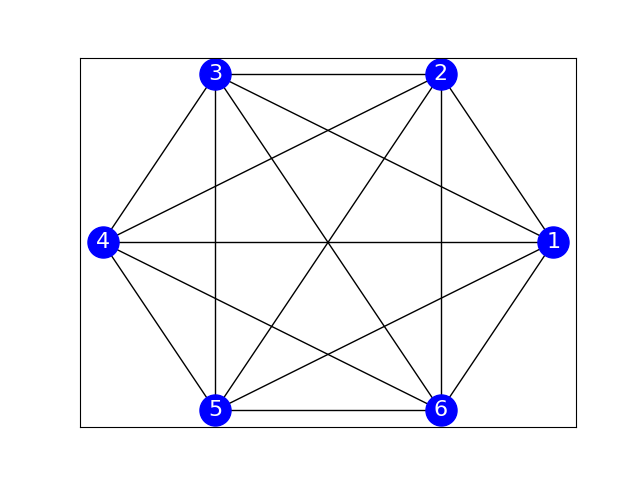
\includegraphics[width=0.6\textwidth]{complete_graph}
\caption{A complete graph with $n=6$ vertices}
\label{fig:my_label} 
\end{figure}

\begin{enumerate}
\item In what order does \texttt{DFS} explore vertices in the above graph?
Assume \texttt{DFS} starts at vertex 4. The adjacency lists are in
ascending order by the numeric label. 

\item[\textbf{Solution:}]  
4, 1, 2, 3, 5, 6

\item What is the running time of \texttt{DFS} on a complete graph with
$n$ vertices? Provide an asymptotic big-oh bound in terms of the
number of vertices. Explain your reasoning. 

\item[\textbf{Solution:}]  
$O(V+E)$ where V is the number of vertices and E is the number of edges. The total number of edges can be written as  $\frac{n(n-1)}{2}$ since the vertices in a complete graph is connected to all other vetices. Therefore $O(V+E)$ can be written as $O(n+\frac{n(n-1)}{2}) = O(n^2)$

\item How many back edges, forward edges, cross edges, and exploratory edges
are generated by running \texttt{DFS} on a complete graph with $n$
vertices? 

\item[\textbf{Solution:}]  
Back Edges: Back edges will be generated by every edge that is not a tree edge. Since tree edges are given by $n-1$, and the total number of edges is given by $\frac{n(n-1)}{2}$. Therefore, back edges are given by $\frac{n(n-1)}{2} - (n-1)$, which is $\frac{n^2-3n-2}{2}$.

Forward Edges: Forward edges are edges that connect a vertex to a descendant in the DFS tree. Since every possible connection exists, every edge that leads to a yet-to-be-visited vertex can be considered a forward edge. However, in the DFS process, each vertex is visited exactly once, and once a vertex is visited, all its edges are explored. Therefore, there are no forward edges in this context.

Cross Edges: Cross edges are edges that are not part of the DFS tree and they connect vertices such that neither is an ancestor of the other in the DFS tree. Since every pair of vertices is connected and DFS visits each vertex exactly once, there are no cross edges.

Exploratory (Tree) Edges: The DFS will generate a total of $n-1$ exploratory edges in a complete graph. This is because in a DFS spanning tree of a connected graph, there are always $V-1$ edges, where $V$ is the number of vertices. 

\end{enumerate}
\pagebreak{}
\item (10 points) Answer each of the following questions with a tight big-O
asymptotic bound. Justify with algorithmic reasoning. 
\begin{enumerate}
\item A priority queue, \texttt{UnsortedMPQ}, is implemented based on an
unsorted array. What is the running time of the operation which retrieves
the minimum value?
\begin{center}
\texttt{unsorted\_min(n)$\in O(\ldots)$}
\par\end{center}

\item[\textbf{Solution:}]
$O(n)$. Since each element would have to be visited exactly once to determine the minimum value of the array. \\

\item Dijkstra's algorithm is implemented based on this unsorted minimum
priority queue. What is the running time of this implementation of
Dijkstra's algorithm?
\begin{center}
\texttt{dijkstra(V,E)$\in O(\dots)$}
\par\end{center}

\item[\textbf{Solution:}]
$O(V^2)$. Since the running time for retriving min element is $O(n)$, and unsorted MPQ is used to implement Dijkstra's algorithm in this case. Each vertex is visited exactly once after extracting the minimum value from the queue, and each vertex that is called visits the number of edges of unvisited vertices. Therefore, the running time of this algorithm is given by $O(V^2+E)$. E in this case, cannot be larger than the number of $V$, $E = V - 1$. So the running time for this algorithm implemented using MPQ is $O(V^2+V-1) = O(V^2)$.

\end{enumerate}
\pagebreak{}
\item (15 points) Find the shortest path from D to all other vertices for
the graph below. 
\begin{center}
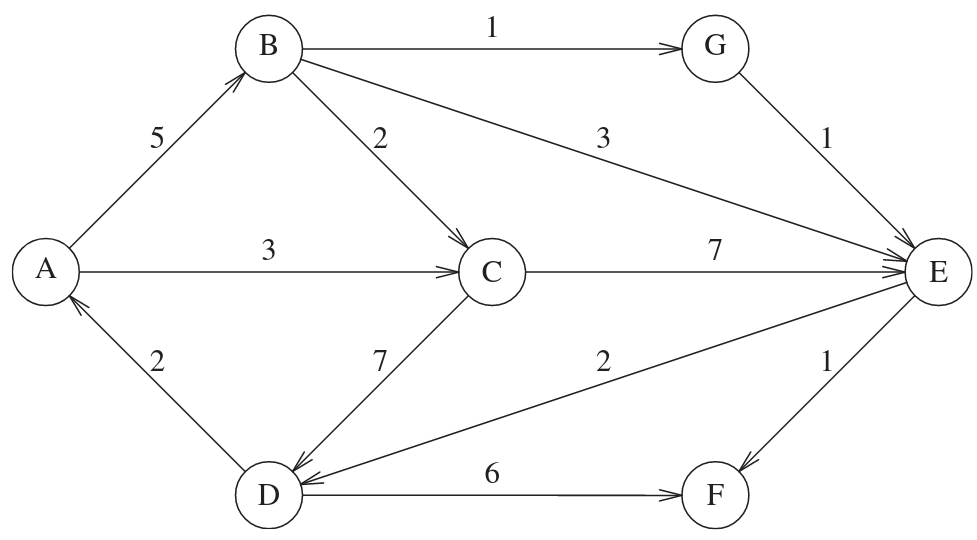
\includegraphics[scale=0.3]{dijkstras_graph}
\par\end{center}
\begin{enumerate}
\item Illustrate the minimum priority queue at each iteration Dijkstra's
algorithm.

\item[\textbf{Solution:}]
\begin{center}
\begin{tabular}{ |c||c|c|c|c|c|c|c|c|c| } 
\hline
\multicolumn{9}{|c|}{MPQ Dijkstra} \\
\hline
num & Pop & A & B & C & D & E & F & G\\
\hline
 0 & - & $\infty$ & $\infty$ & $\infty$ & 0 & $\infty$ & $\infty$ & $\infty$ \\ 
 1 & D & $2^D$ & $\infty$ & $\infty$ &  & $\infty$ & $6^D$ & $\infty$ \\ 
 2 & A &  & $7^A$ & $5^A$ &  & $\infty$ & $6^D$ & $\infty$ \\ 
 3 & C &  & $7^A$ &  &  & $12^C$ & $6^D$ & $\infty$ \\ 
 4 & F &  & $7^A$ &  &  & $12^C$ &  & $\infty$ \\ 
 5 & B &  &  &  &  & $10^B$ &  & $8^B$ \\ 
 6 & G &  &  &  &  & $9^G$ &  & \\ 
 7 & E &  &  &  &  &  &  & \\ 
 \hline
\end{tabular}
\end{center}
\item Draw the Shortest Path Tree.

\item[\textbf{Solution:}]

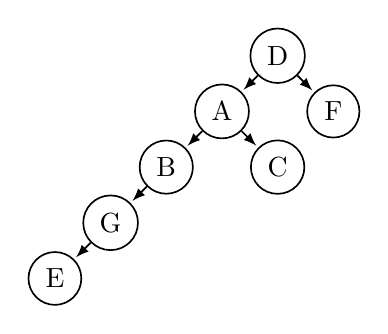
\begin{tikzpicture}[->,>=stealth,shorten >=1pt,auto,node distance=1cm, semithick]
  \tikzset{vertex/.style = {shape=circle,draw,minimum size=1em}}
  \tikzset{edge/.style = {->,> = latex}}

  \node[vertex] (D)                         {D};
  \node[vertex] (A) [below left of=D]  {A};
  \node[vertex] (F) [below right of=D] {F};
  \node[vertex] (B) [below left of=A]  {B};
  \node[vertex] (C) [below right of=A] {C};
  \node[vertex] (G) [below left of=B]   {G};
  \node[vertex] (E) [below left of=G]   {E};

  \draw[edge] (D) to (A);
  \draw[edge] (D) to (F);
  \draw[edge] (A) to (B);
  \draw[edge] (A) to (C);
  \draw[edge] (B) to (G);
  \draw[edge] (G) to (E);
\end{tikzpicture}

\item What is the running time of the Dijkstra's algorithm under the assumption that the graph is implemented based on an adjacency list and the minimum priority queue is implemented based on a binary heap?

\item[\textbf{Solution:}]
The running time of Dijkstra's algorithm under these assumptions are $O((V+E) log V)$ where $V$ is the number of vertices and $E$ is the number of edges.
Initialization of each vertex in a graph takes $O(V)$ total. Using Minimum Priority Queue to extact each elements takes total of $O(Vlog V)$. The relax function is called for every adjacent edges of a vertex, which is $O(ElogV)$. The total running time is $O((V+E)logV)$.

\end{enumerate}
\pagebreak{}
\item (15 points) Find the shortest path from vertex 3 to all other vertices for the graph below. 
\begin{center}
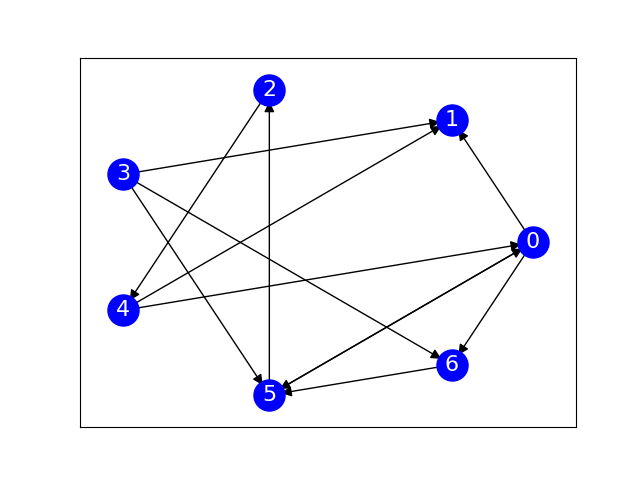
\includegraphics[scale=0.6]{undirected}
\par\end{center}
\begin{enumerate}
\item Which graph algorithm can solve the problem most \emph{efficiently}?

\item[\textbf{Solution:}]
BFS.

\item How could you use the same algorithm if the graph had edge weights?
(\textit{Hint}: You may want to create intermediate nodes.)

\item[\textbf{Solution:}]
Using intermediate nodes, for each edge in the original graph with a weight greater than 1, introduce intermediate nodes to break the edge into several edges of weight 1. For example, if there's an edge of weight 3 between Node A and Node B, you would remove this edge and add two intermediate nodes, X and Y. You would then create edges A-X, X-Y, and Y-B, each with a weight of 1. After Transforming all the edges into weights of 1, apply BFS on the new graph, then transform the path with intermediate nodes removed.

\item Draw the Shortest Path Tree.

\item[\textbf{Solution:}]
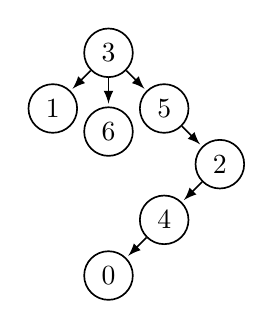
\begin{tikzpicture}[->,>=stealth,shorten >=1pt,auto,node distance=1cm, semithick]
  \tikzset{vertex/.style = {shape=circle,draw,minimum size=1em}}
  \tikzset{edge/.style = {->,> = latex}}

  \node[vertex] (3)                         {3};
  \node[vertex] (1) [below left of=3]  {1};
  \node[vertex] (5) [below right of=3] {5};
  \node[vertex] (6) [below of=3]  {6};
  \node[vertex] (2) [below right of=5] {2};
  \node[vertex] (4) [below left of=2]   {4};
  \node[vertex] (0) [below left of=4]   {0};

  \draw[edge] (3) to (1);
  \draw[edge] (3) to (5);
  \draw[edge] (3) to (6);
  \draw[edge] (5) to (2);
  \draw[edge] (2) to (4);
  \draw[edge] (4) to (0);
\end{tikzpicture}

\end{enumerate}
\pagebreak{}
\item (15 points) There are five small islands in a lake, and the state
wants to build four bridges to connect them so that each island can
be reached from any other one via one or more bridges. The cost of
bridge construction is proportional to its length. The distance between
pairs of islands are given in the following table. 

\begin{table}[H]
\centering{}%
\begin{tabular}{cccccc}
 & 1  & 2  & 3  & 4  & 5 \tabularnewline
1  & -  & 10  & 15  & 10  & 20 \tabularnewline
2  & -  & -  & 15  & 20  & 20 \tabularnewline
3  & -  & -  & -  & 15  & 30 \tabularnewline
4  & -  & -  & -  & -  & 10 \tabularnewline
5  & -  & -  & -  & -  & - \tabularnewline
\end{tabular}\caption{The distance between any two islands}
\label{tab:islands_graph} 
\end{table}

\begin{figure}[H]
\centering{}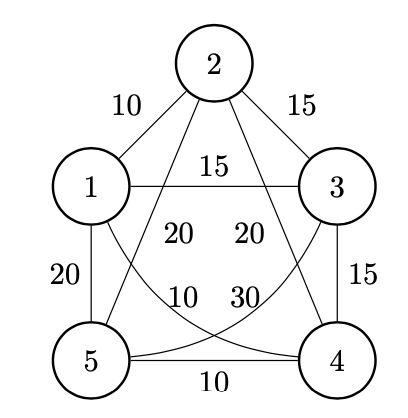
\includegraphics[scale=0.8]{island_graph_distances}\caption{The distance between any two islands}
\label{fig:islands_graph} 
\end{figure}

\begin{enumerate}
\item Illustrate the steps of Prim's algorithm using the graph above. Draw the Minimum Spanning Tree. What is the length of the bridges?

\item[\textbf{Solution:}]
Using Prim's algoritm:\\
1. Start with any vertex: Let's start with island 1.\\
2. Choose the smallest edge connecting to a new vertex: The smallest edge from island 1 is to island 2 (10 units).\\
3. Repeat the process: Now, we consider the edges from both island 1 and island 4.\\
4. Keep adding the smallest edge that connects a new vertex: Continue this process until all vertices are included.\\
The total length of bridges is $10 + 10 + 10 + 15 = 45$.\\
\begin{center}
\begin{tabular}{ |c||c|c|c|c|c|c| } 
\hline
\multicolumn{7}{|c|}{Prim} \\
\hline
 & Pop & 1 & 2 & 3 & 4 & 5 \\
\hline \hline
1  & (1,2) & -  & 10  & 15  & 10  & 20 \tabularnewline
2  & (2,3) & -  & -  & 15  & 20  & 20 \tabularnewline
3  & (1,4) & -  & -  & -  & 15  & 30 \tabularnewline
4  & (4,5) & -  & -  & -  & -  & 10 \tabularnewline
5  & & -  & -  & -  & -  & - \tabularnewline
 \hline
\end{tabular}
\end{center}

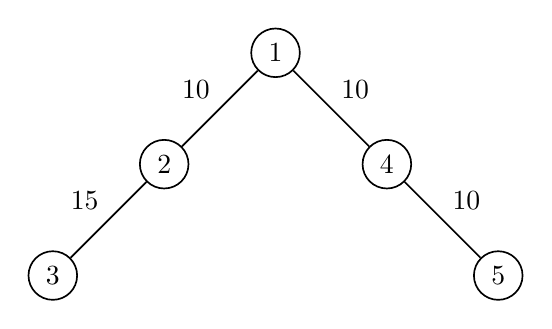
\begin{tikzpicture}[auto, node distance=2cm, semithick]
  \tikzset{vertex/.style = {shape=circle,draw,minimum size=1em}}
  \tikzset{edge/.style = {>=latex}}

  \node[vertex] (1)                     {1};
  \node[vertex] (2) [below left of=1]  {2};
  \node[vertex] (3) [below left of=2] {3};
  \node[vertex] (4) [below right of=1] {4};
  \node[vertex] (5) [below right of=4] {5};

  \draw[edge] (1) -- node[above right] {10} (4);
  \draw[edge] (4) -- node[above right] {10} (5);
  \draw[edge] (1) -- node[above left] {10} (2);
  \draw[edge] (2) -- node[above left] {15} (3);
\end{tikzpicture}

\item Illustrate the steps of Kruskal's algorithm using the graph above. Draw the Minimum Spanning Tree. What is the length of the bridges?

\item[\textbf{Solution:}]
Using Kruskal's Algorithm:\\
1. Sort all the edges by length:\\
\{(1,2): 10, (1,4): 10, (4,5): 10, (1,3): 15, (2,3): 15, (3,4): 15, (1,5); 20, (2,5): 20, (3,5): 30 \}\\
2. Add the shortest edge, (1,4): 10 to the MST.
3. Add the next shortest edge without forming a cycle to the MST,  $(4,5): 10$ and $(1,2): 10$. Since (1,3) creates a cycle with $(1,2)$ and $(1,3)$.\\
4. Add the final edge to connect all the islands, $(2,3): 15$.
The total length of bridges is also $10 + 10 + 10 + 15 = 45$.
\begin{center}
\begin{tabular}{ |c||c|c|c|c|c|c|c|c|c| } 
\hline
\multicolumn{10}{|c|}{Kruskal} \\
\hline
 & (1,2) & (1,4) & (4,5) & (1,3) & (2,3) & (3,4) & (1,5) & (2,5) & (3,5) \\
\hline \hline
Weight  & 10 & 10  & 10  & 15  & 15  & 15 & 20 & 20 & 30 \tabularnewline
Insertion & Y & Y & Y & N & Y & N & N & N & N \tabularnewline
Order & 1 & 2 & 3 &  & 4 &  &  &  &  \tabularnewline
 \hline
\end{tabular}
\end{center}

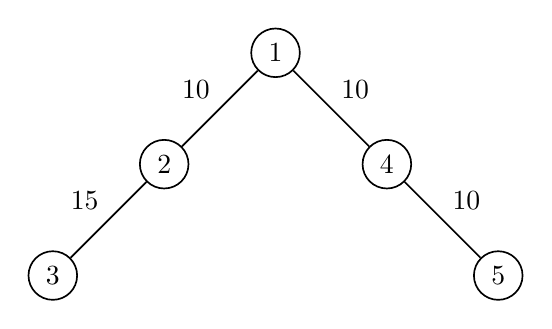
\begin{tikzpicture}[auto, node distance=2cm, semithick]
  \tikzset{vertex/.style = {shape=circle,draw,minimum size=1em}}
  \tikzset{edge/.style = {>=latex}}

  \node[vertex] (1)                     {1};
  \node[vertex] (2) [below left of=1]  {2};
  \node[vertex] (3) [below left of=2] {3};
  \node[vertex] (4) [below right of=1] {4};
  \node[vertex] (5) [below right of=4] {5};

  \draw[edge] (1) -- node[above right] {10} (4);
  \draw[edge] (4) -- node[above right] {10} (5);
  \draw[edge] (1) -- node[above left] {10} (2);
  \draw[edge] (2) -- node[above left] {15} (3);
\end{tikzpicture}

\end{enumerate}
\end{enumerate}

\end{document}
